\documentclass[9pt]{beamer}
\usepackage[utf8]{inputenc}
\usepackage{floatrow}
\usepackage{color}

\usepackage{tikz}
\usetikzlibrary{shapes,arrows}

\graphicspath{ {img/} }

\makeatletter
\newcommand*{\currentname}{\@currentlabelname}
\makeatother

\usetheme{Boadilla}
\usecolortheme{whale}
\beamertemplatenavigationsymbolsempty 
\setbeamersize{text margin left=1em,text margin right=1em}

\AtBeginSection[]
{
  \begin{frame}
    \frametitle{Table of Contents}
		\setcounter{tocdepth}{2}
    \tableofcontents[currentsection]
  \end{frame}
}

\title{myTaxiService}
\subtitle{Final Presentation}
\author{Jacopo Strada, Luca Riva}
\date{February 26, 2016}
\institute[]{Politecnico di Milano\\Software Engineering 2 Project}

\begin{document}

\maketitle

% REQUIREMENTS AND SPECIFICATION
\section{Requirement And Specification}


\subsection{Scope}

\begin{frame}{\currentname}

The \emph{myTaxiService} software focuses on helping the clients benefit from the service and ensures a fair management of taxi queues.

\vfill

\begin{columns}[c]
  \begin{column}{.5\textwidth}
    The software will:
    \begin{itemize}
    \item give the possibility to request a taxi either through a web application or a mobile app.
    \item compute the distribution of taxis in the various zones based on the GPS information it receives from each taxi.
    \item offer programmatic interfaces to enable the development of additional services.
    \item allow to book a taxi by specifying the origin and the destination of the ride.
    \end{itemize}
  \end{column}
  \begin{column}{.47\textwidth}
    
\includegraphics[width=\textwidth]{taxi-cab}
		\centering
  \end{column}
\end{columns}

\end{frame}

\subsection{User Interfaces}

\subsubsection{Clients' User Interfaces}
\begin{frame}{\currentname{}}
\begin{columns}[c]
  \begin{column}{.5\textwidth}
		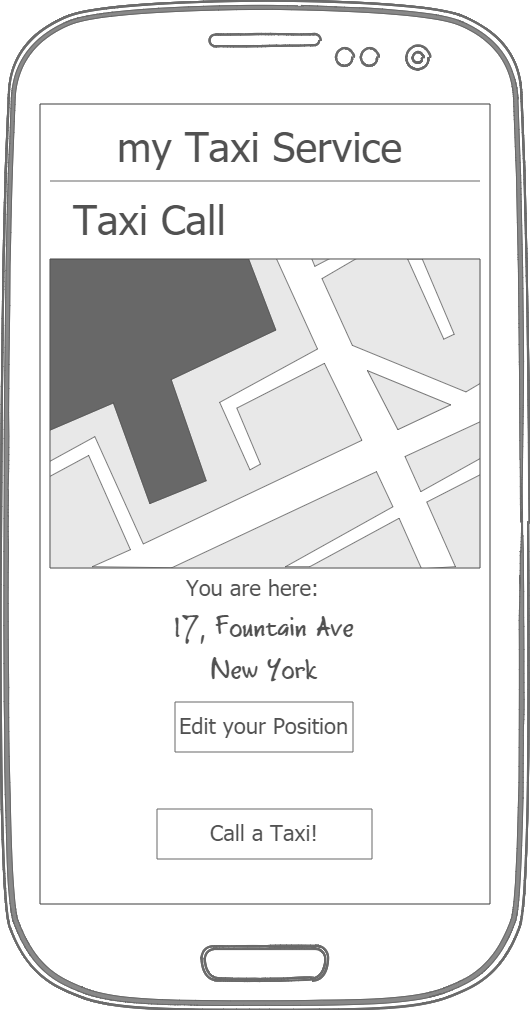
\includegraphics[height=.8\textheight]{Mockup-ClientsTaxiCall}
		\centering
  \end{column}
  \begin{column}{.5\textwidth}
    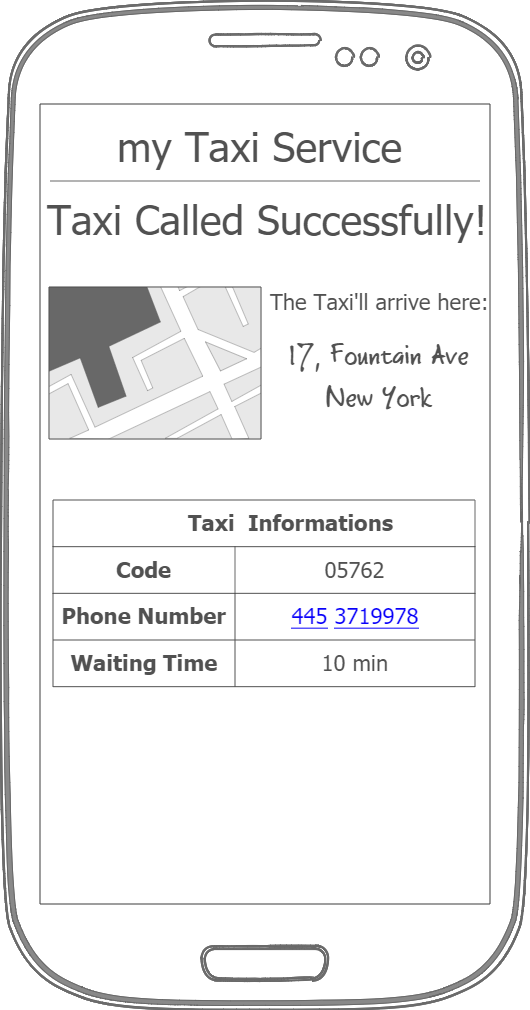
\includegraphics[height=.8\textheight]{Mockup-ClientsTaxiCallConfirmation}
		\centering
  \end{column}
\end{columns}
\end{frame}

\subsubsection{Taxi Drivers' User Interfaces}
\begin{frame}{\currentname{}}
\begin{columns}[c]
  \begin{column}{.5\textwidth}
		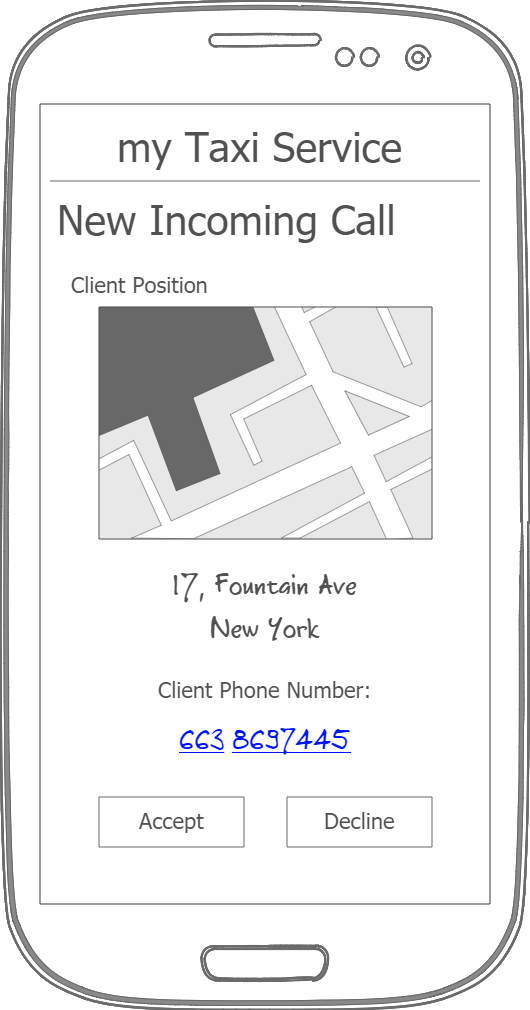
\includegraphics[height=.8\textheight]{Mockup-TaxiDriversNewIncomingCall}
		\centering
  \end{column}
  \begin{column}{.5\textwidth}
    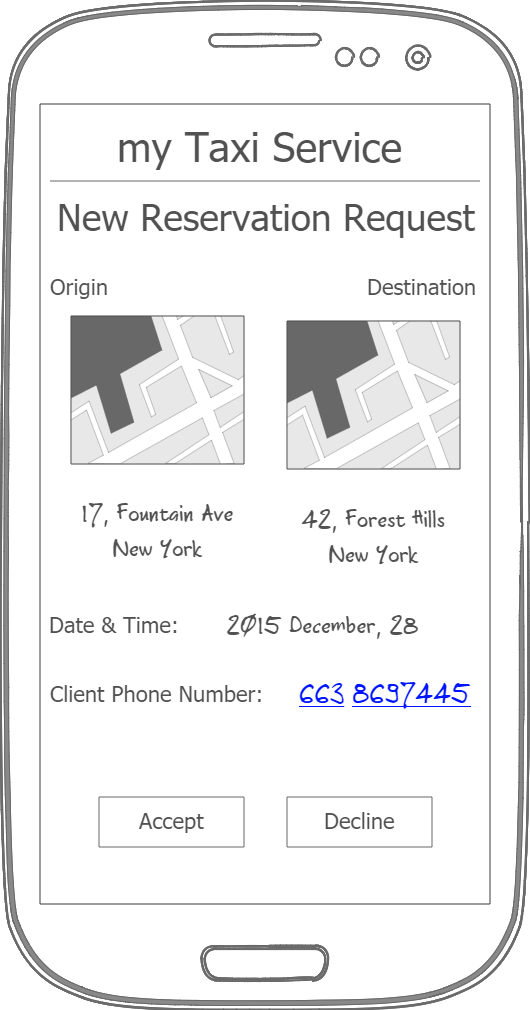
\includegraphics[height=.8\textheight]{Mockup-TaxiDriversReservationRequest}
		\centering
  \end{column}
\end{columns}
\end{frame}

\subsection {The World and The Machine}

\begin{frame}{\currentname}

\begin{figure}[H]
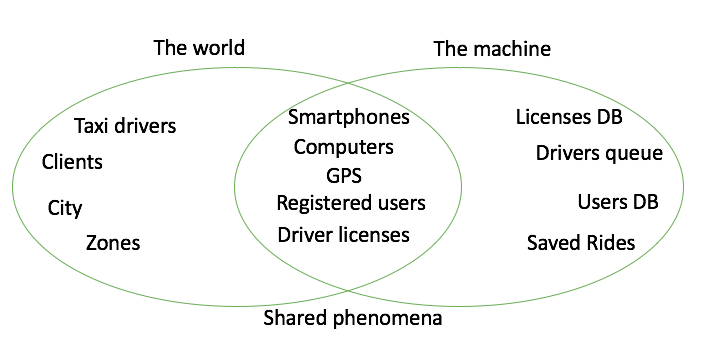
\includegraphics[width=.9\textwidth]{WorldAndMachine}
\centering
\end{figure}

\end{frame}

\subsection{Use Cases}

\begin{frame}{\currentname}

\framesubtitle{Client}

\begin{figure}[H]
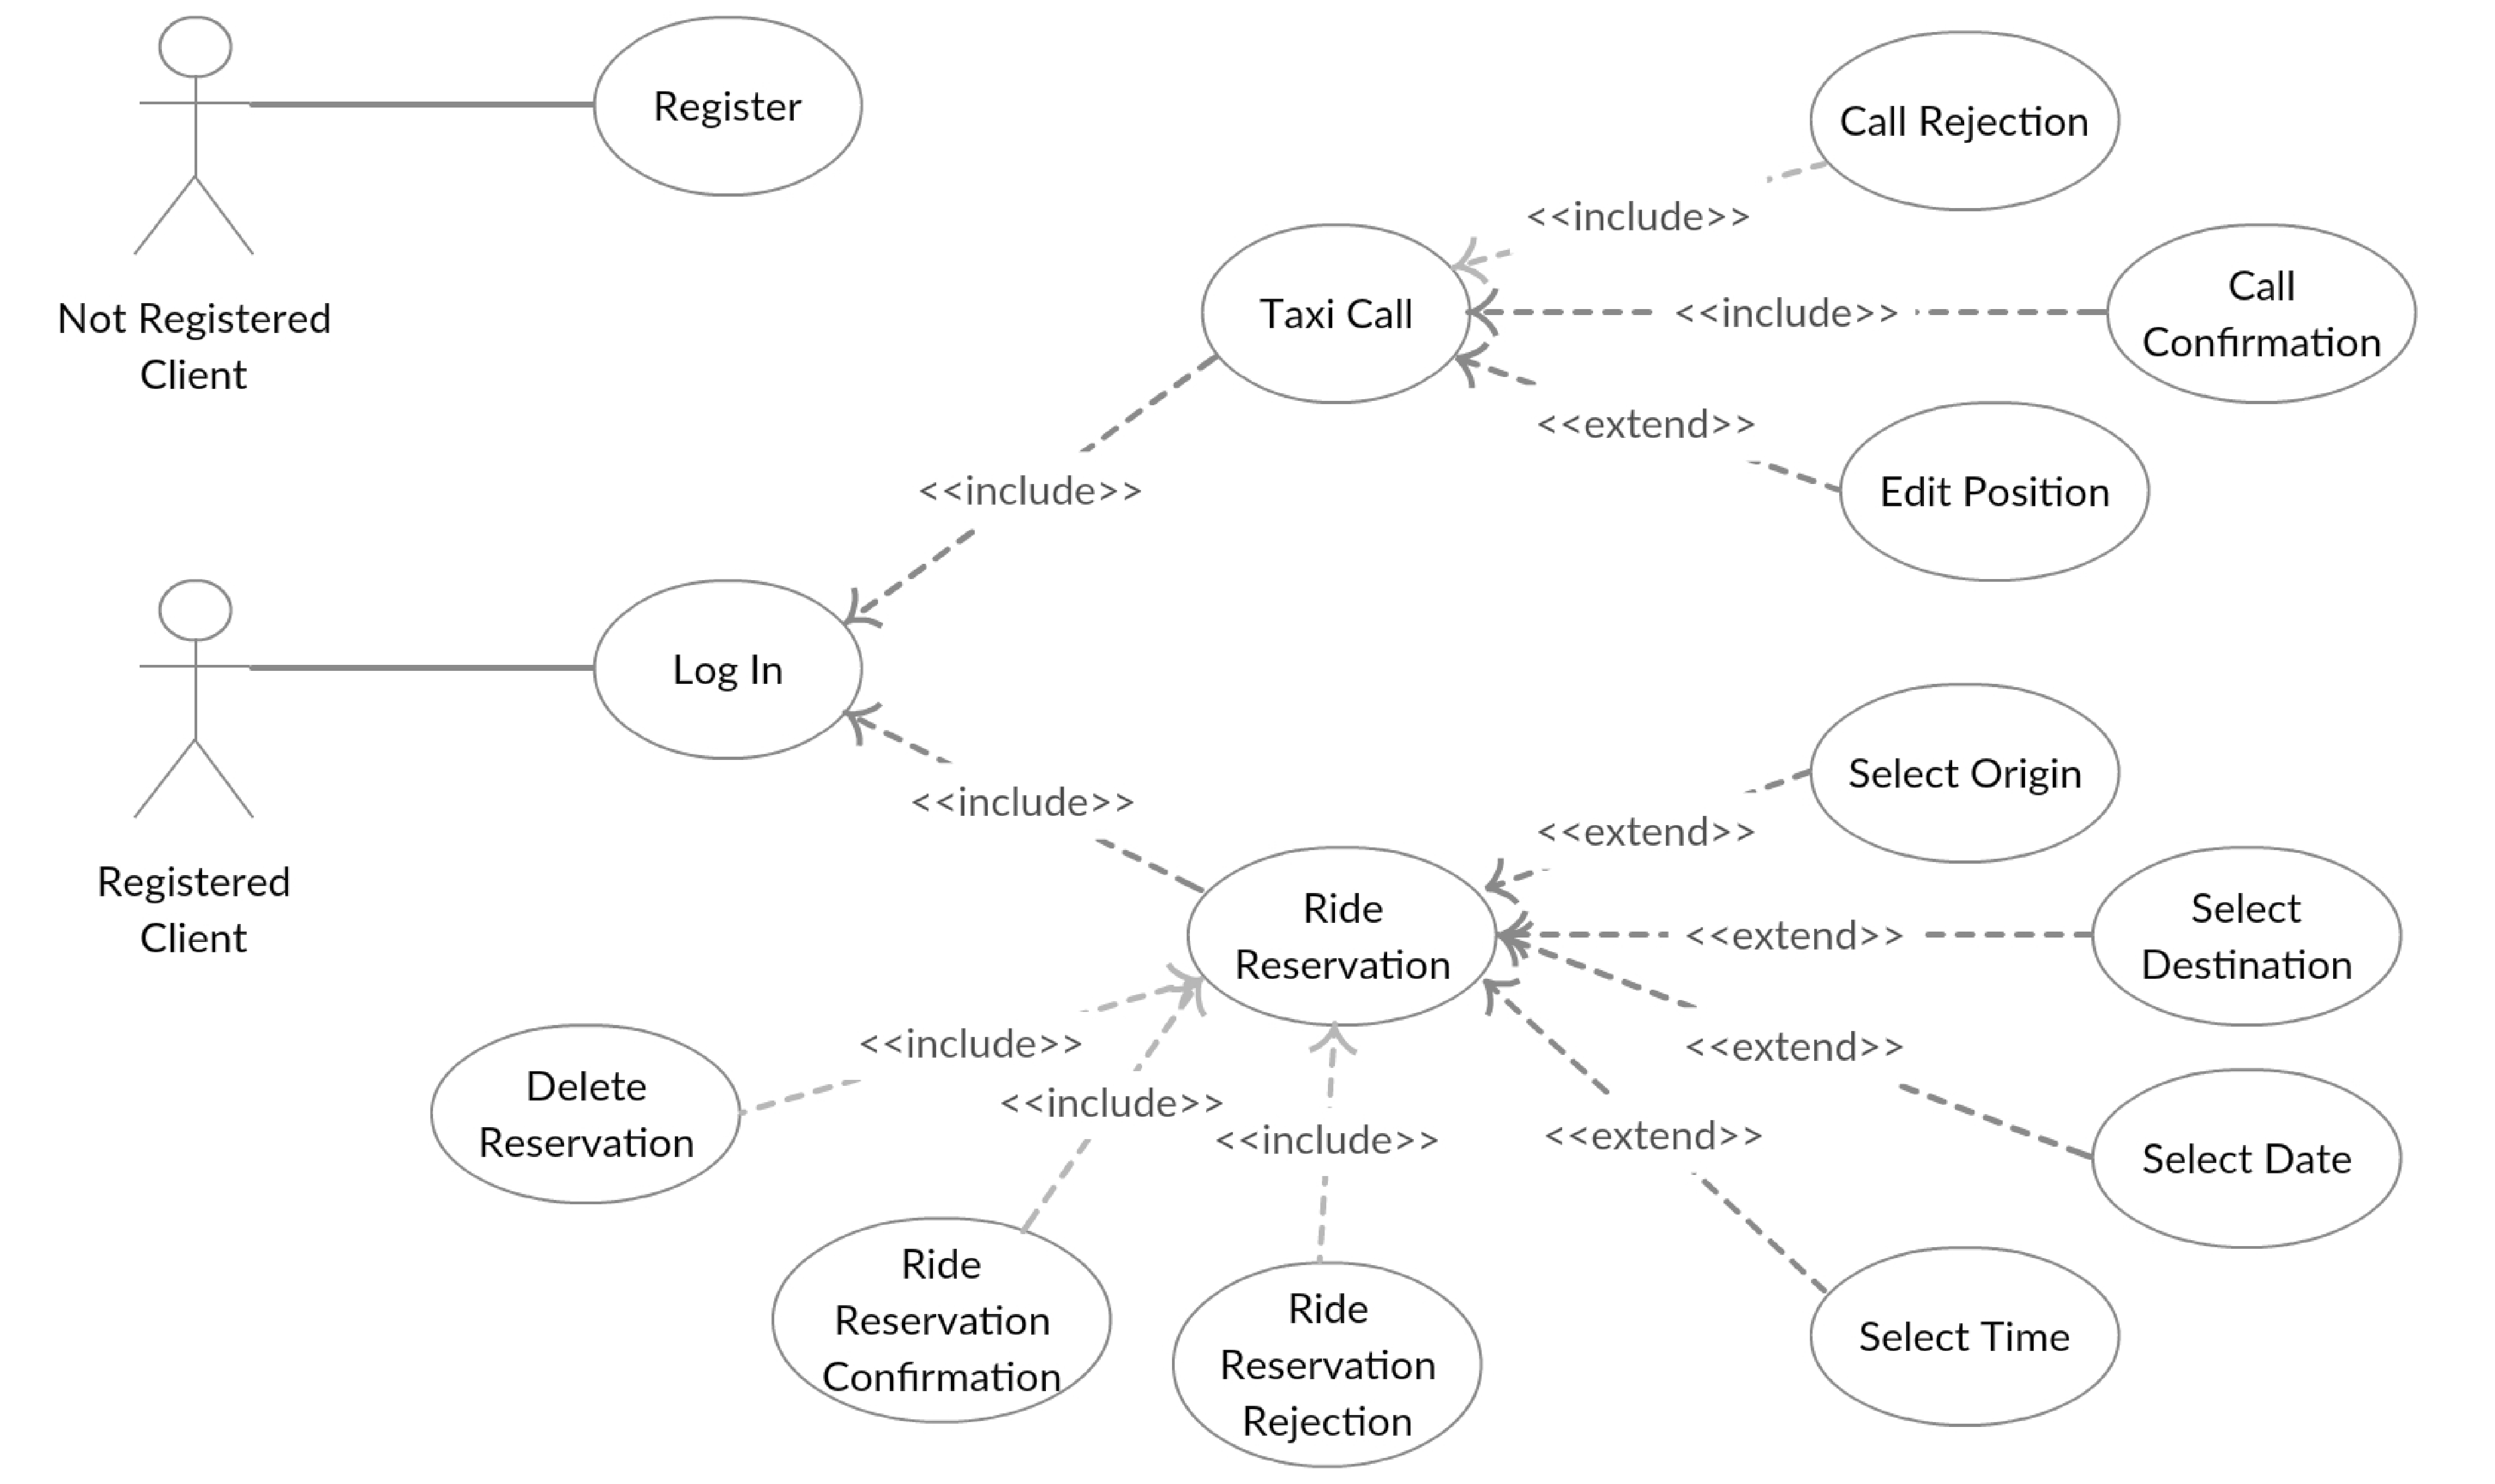
\includegraphics[width=.9\textwidth]{UseCase-Client}
\centering
\end{figure}

\end{frame}

\begin{frame}{\currentname}

\framesubtitle{Taxi Driver}

\begin{figure}[H]
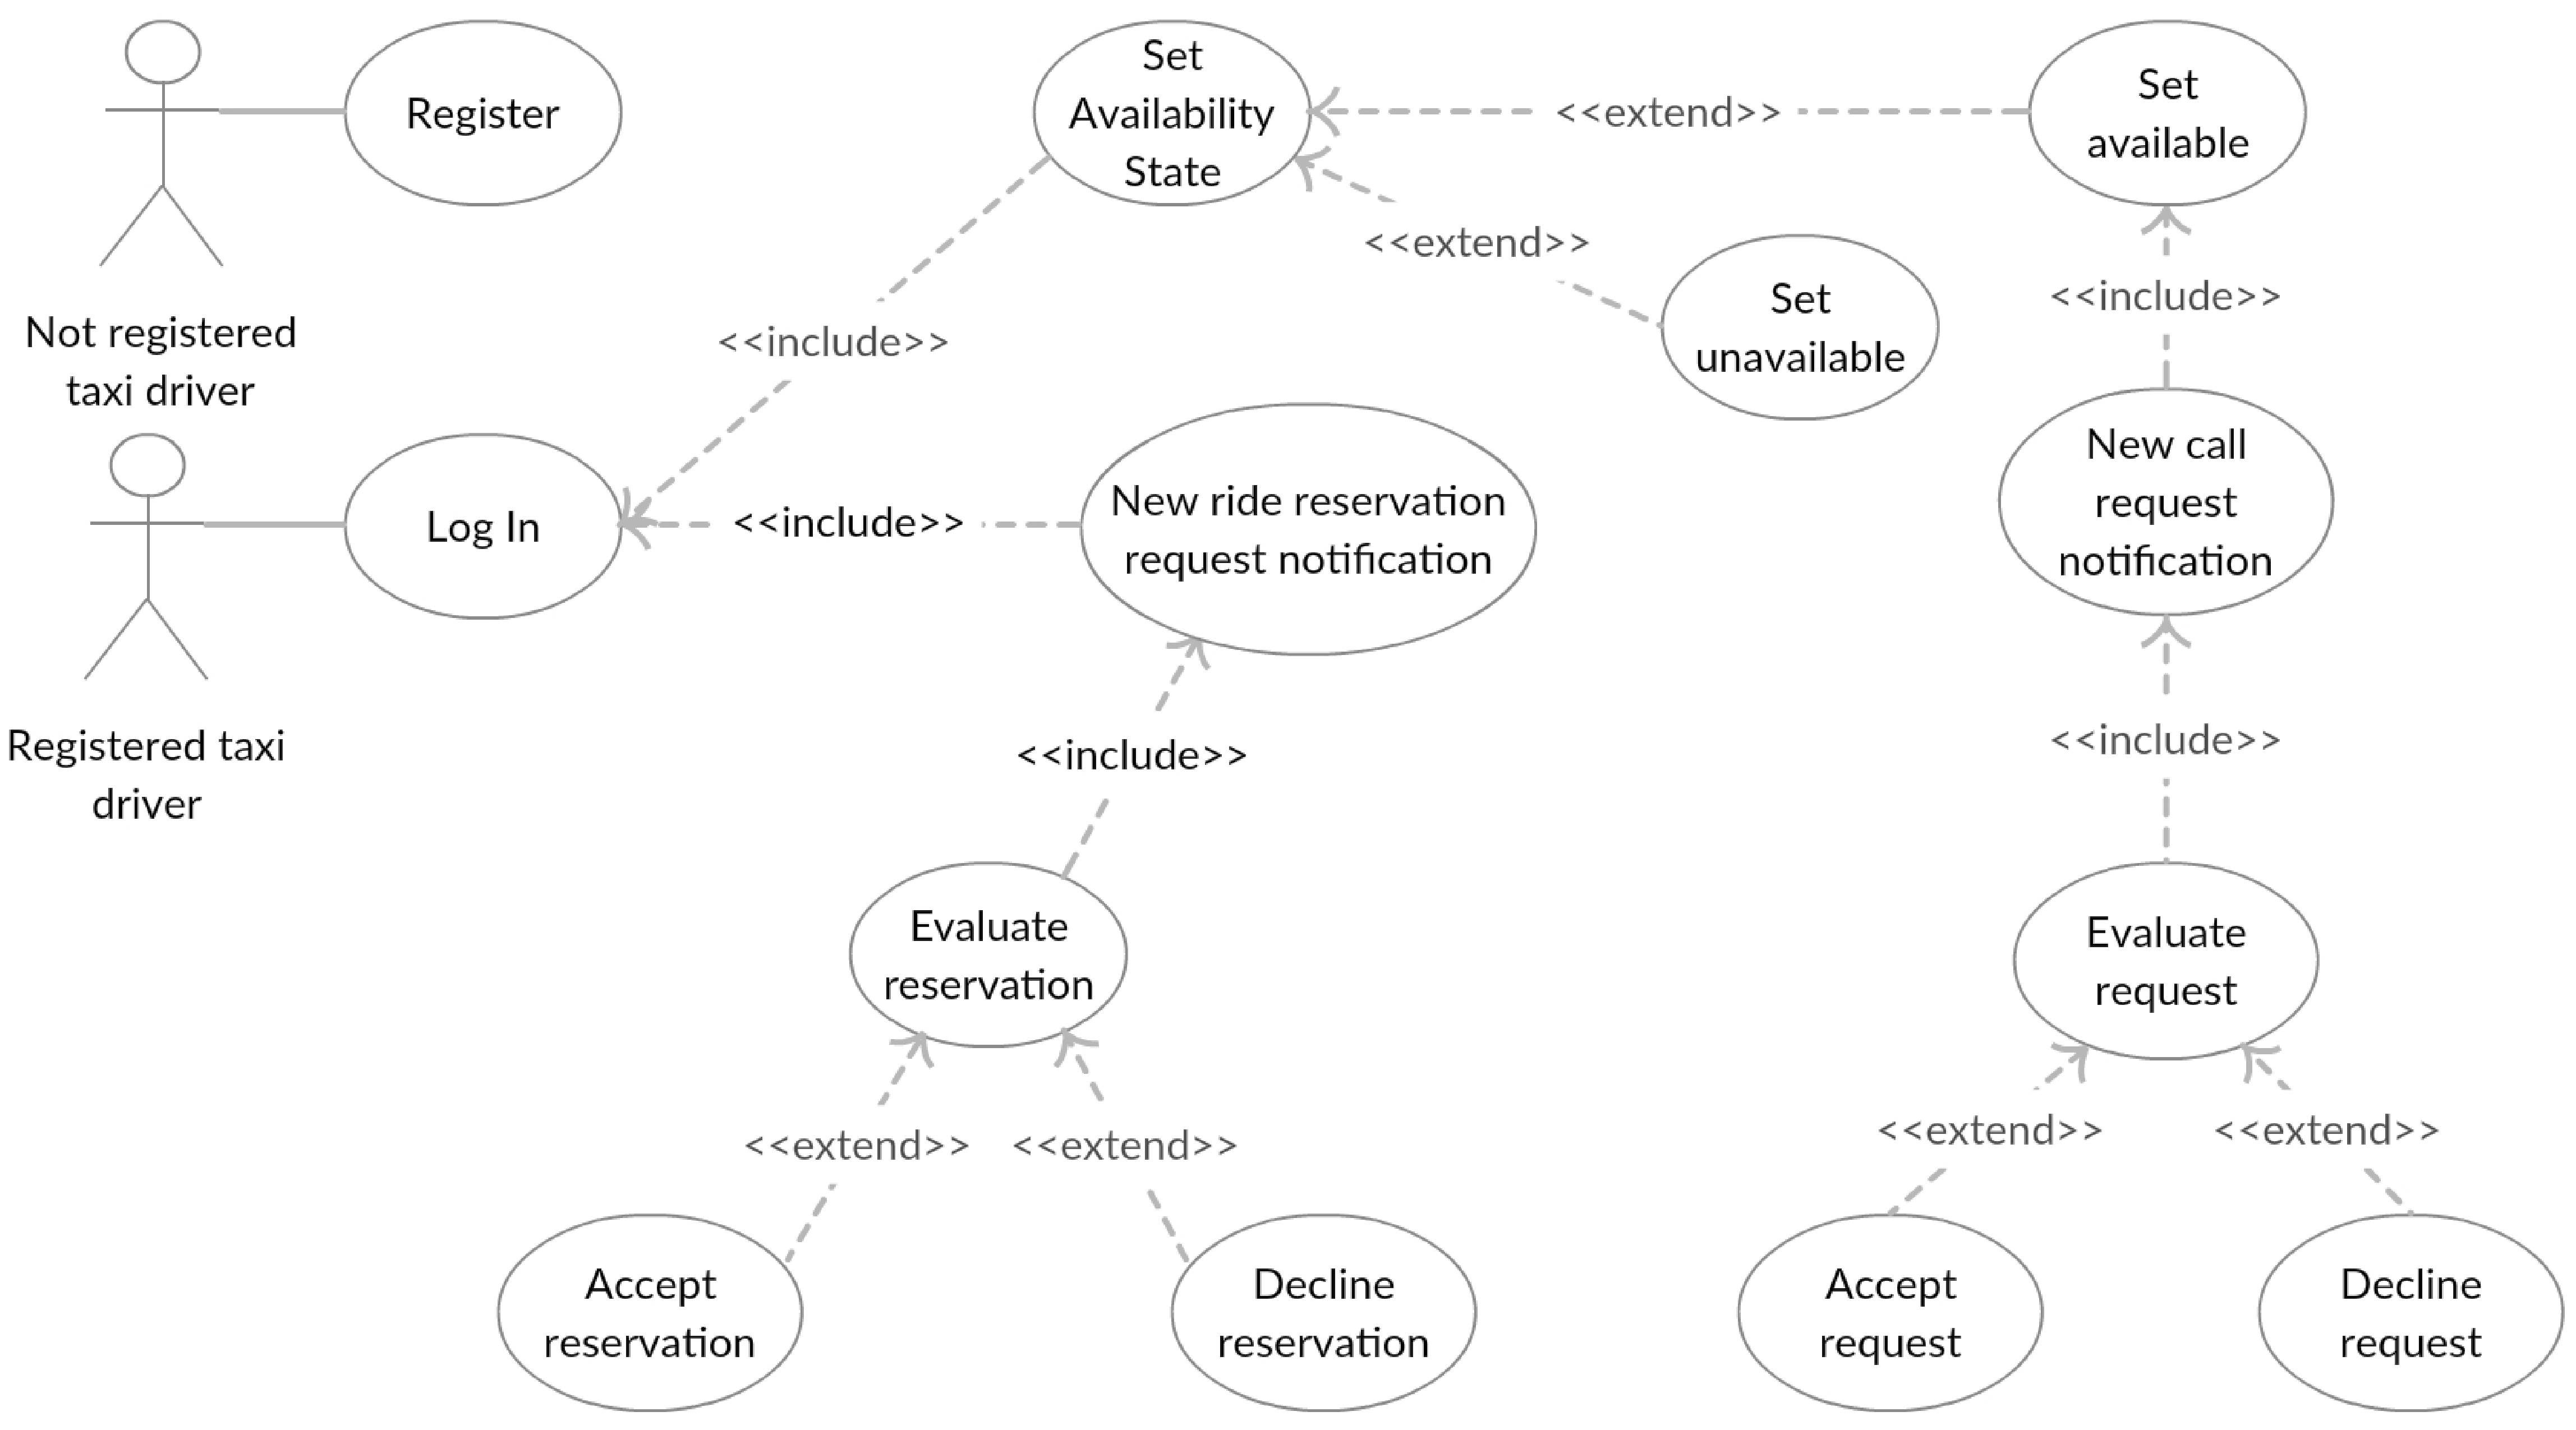
\includegraphics[width=.9\textwidth]{UseCase-TaxiDriver}
\centering
\end{figure}

\end{frame}

\subsection {Alloy}

\begin{frame}{\currentname}

\begin{figure}[H]
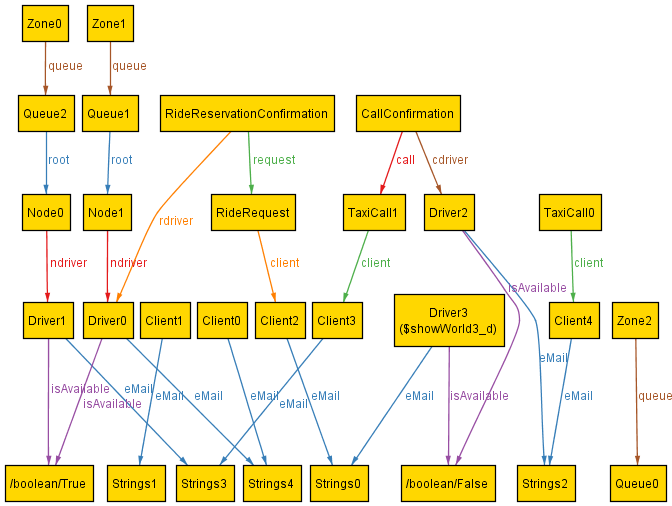
\includegraphics[height=.8\textheight]{Alloy-FreeDriver}
\centering
\end{figure}

\end{frame}

% DESIGN
\section{Design}

\subsection{Component View}

\begin{frame}{\currentname}

\begin{columns}[c]
  \begin{column}{.4\textwidth}
    \begin{small}\textbf{Data Base:} Store all the information about users, zones, queues, drivers position and state, reservations \ldots
        
        \textbf{Account Manager:} Logins and registrations (check all the constraint). Change drivers state.
        
        \textbf{Call Manager:} Get the correct zone from the client position, find an available driver and send a confirmation to the client.
        
        \textbf{Queue Manager:} Provide the first driver in a queue given a zone and manages drivers adding, removing add moving to the end.
        
        \textbf{Reservation Manager:} Checks if a reservation is valid and when a driver accepts it, the reservation is stored in the database.
        
        \textbf{Notification Manager:} Employed for sending notifications to drivers and clients.
        
        \textbf{Position Utilities:} Return a zone from an address, calculate an estimated time for a call or validate a path for a reservation.
        
    \end{small}
  \end{column}
  \begin{column}{.6\textwidth}
    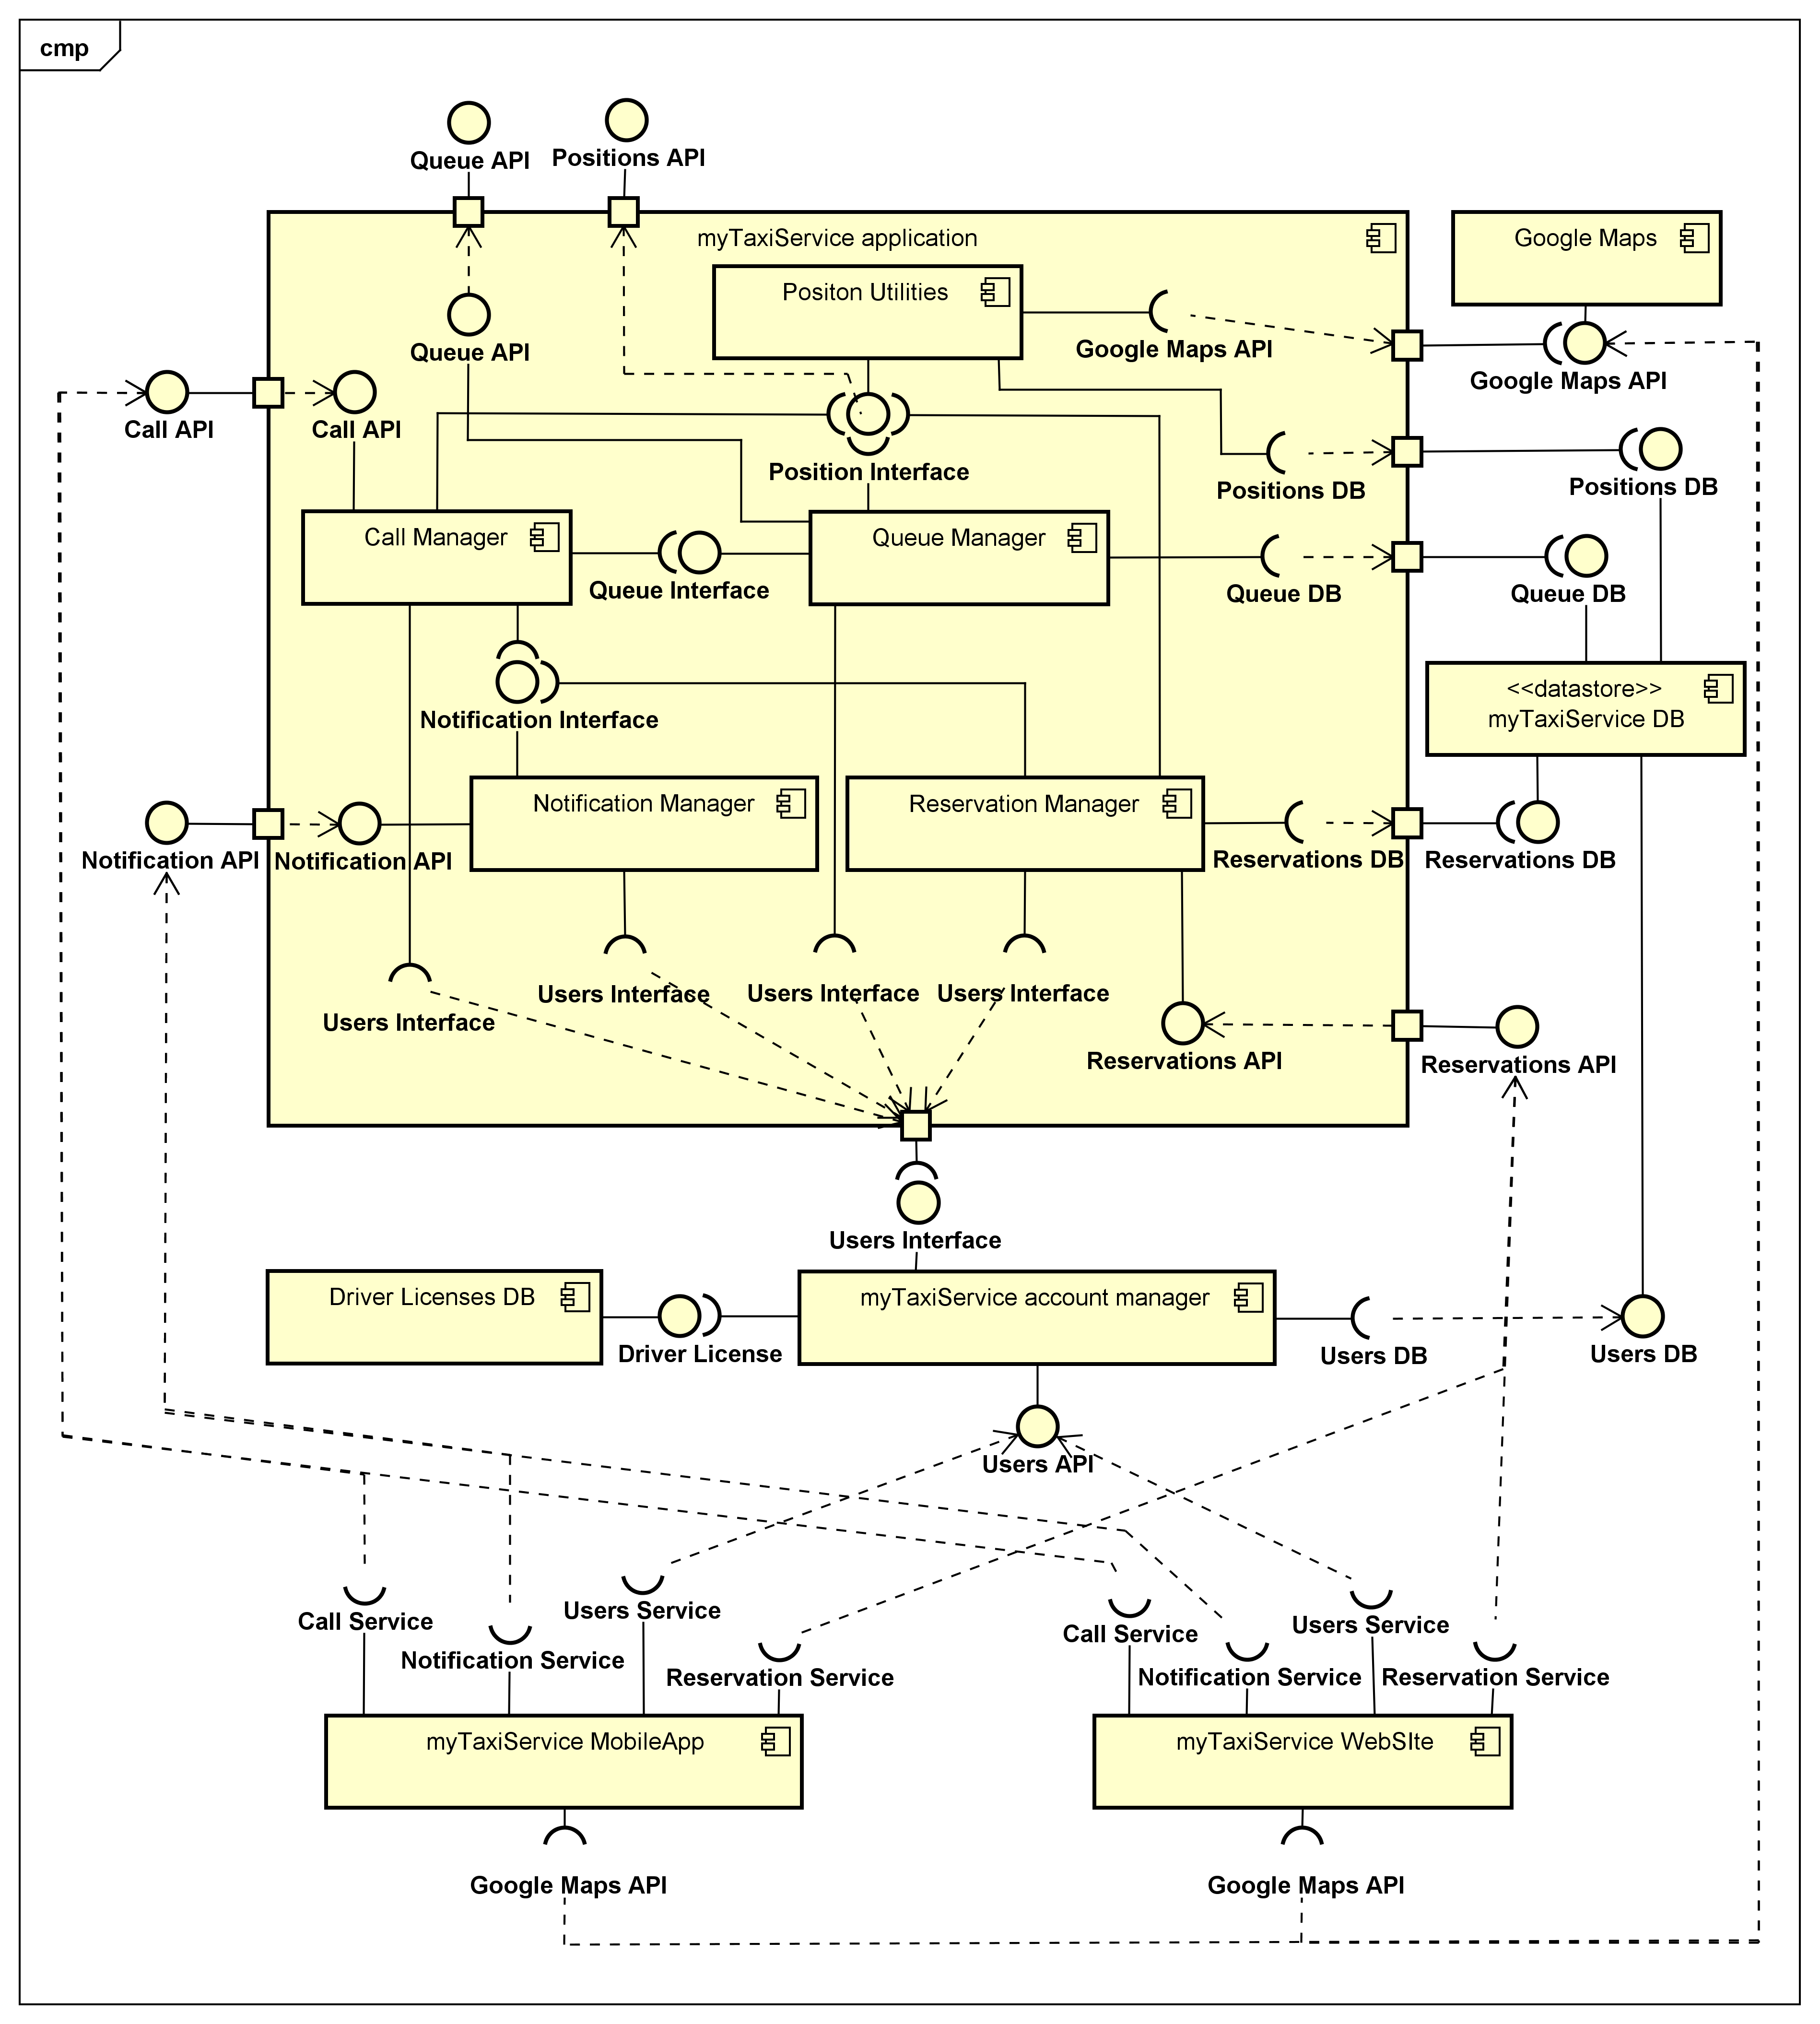
\includegraphics[width=\textwidth]{ComponentDiagram}
	\centering
  \end{column}
\end{columns}

\end{frame}

\subsection{Architectural Style}

\begin{frame}[allowframebreaks]{\currentname}

The system was designed with a \emph{three-tier} architecture: Data, Application Logic and GUI are separated and there are two levels of firewalls in order to keep a high level of security.

\begin{figure}[H]
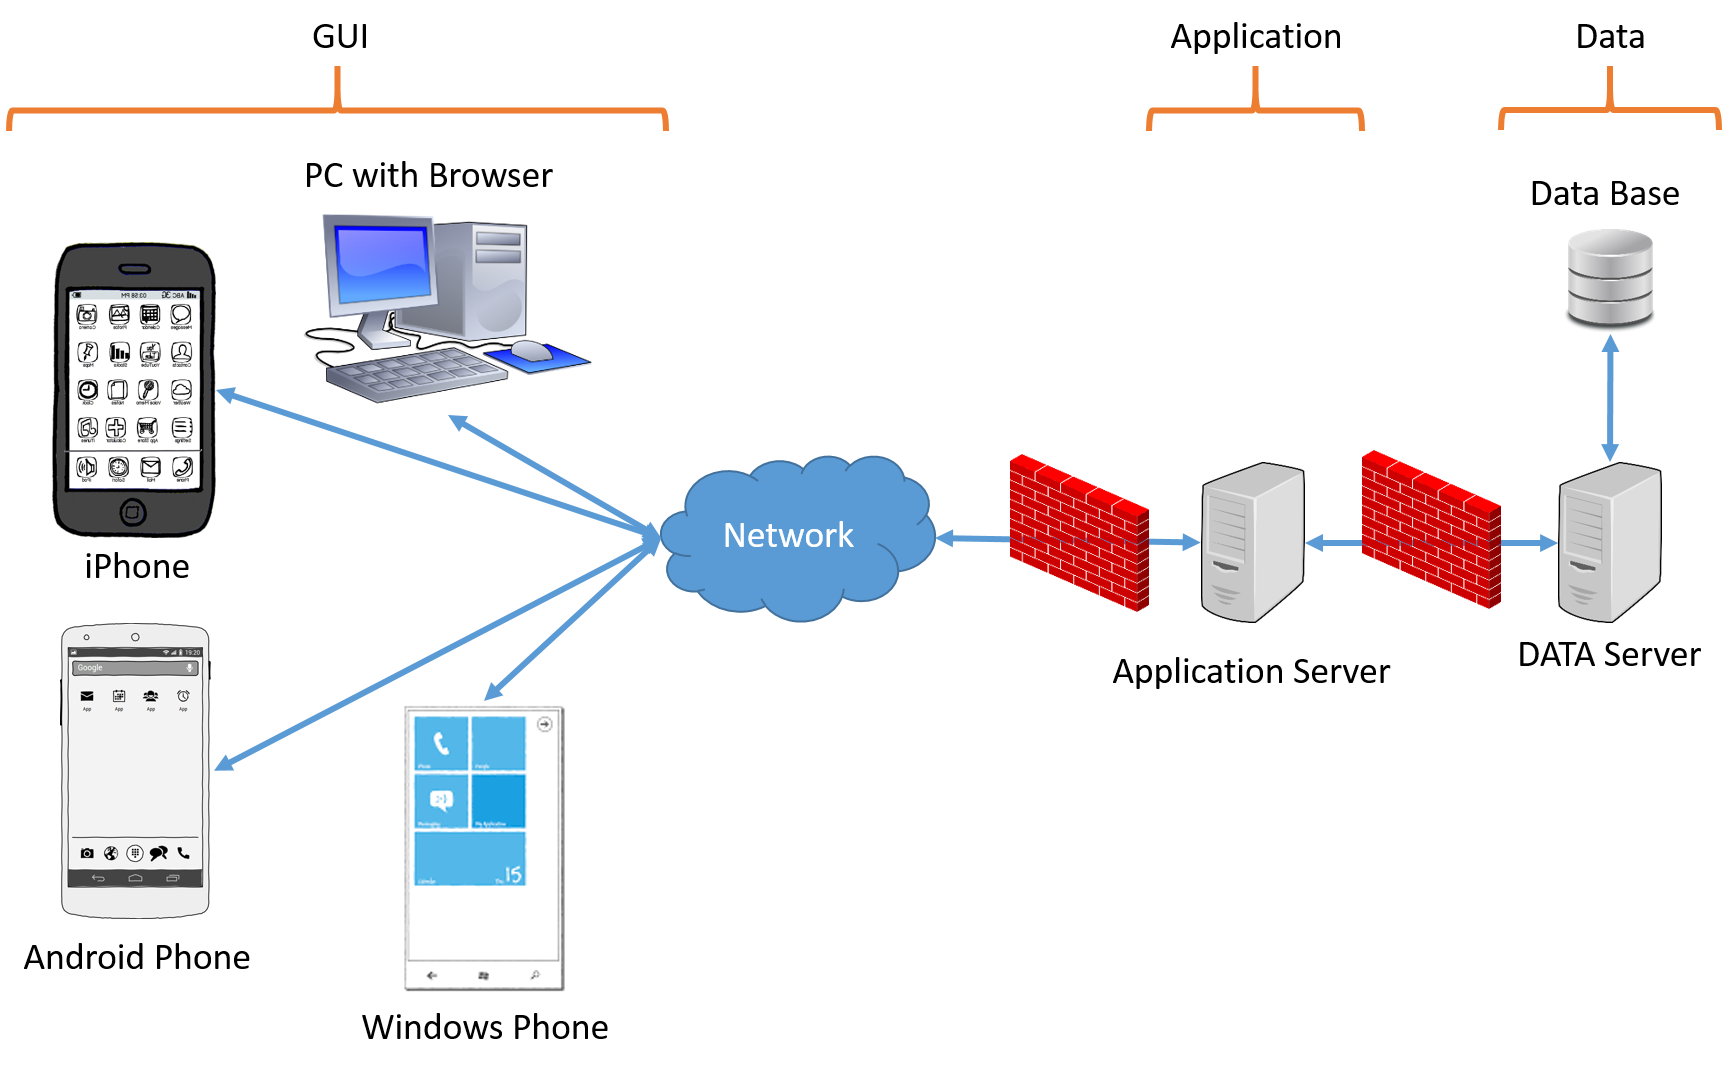
\includegraphics[height=.6\textheight]{Architecture}
\centering
\end{figure}

The \textbf{client server} is used for all the communications which are composed by a request, made by the client, and a response, given by the server.

The \textbf{publisher-subscriber} is needed for the notification service.

\begin{figure}[H]
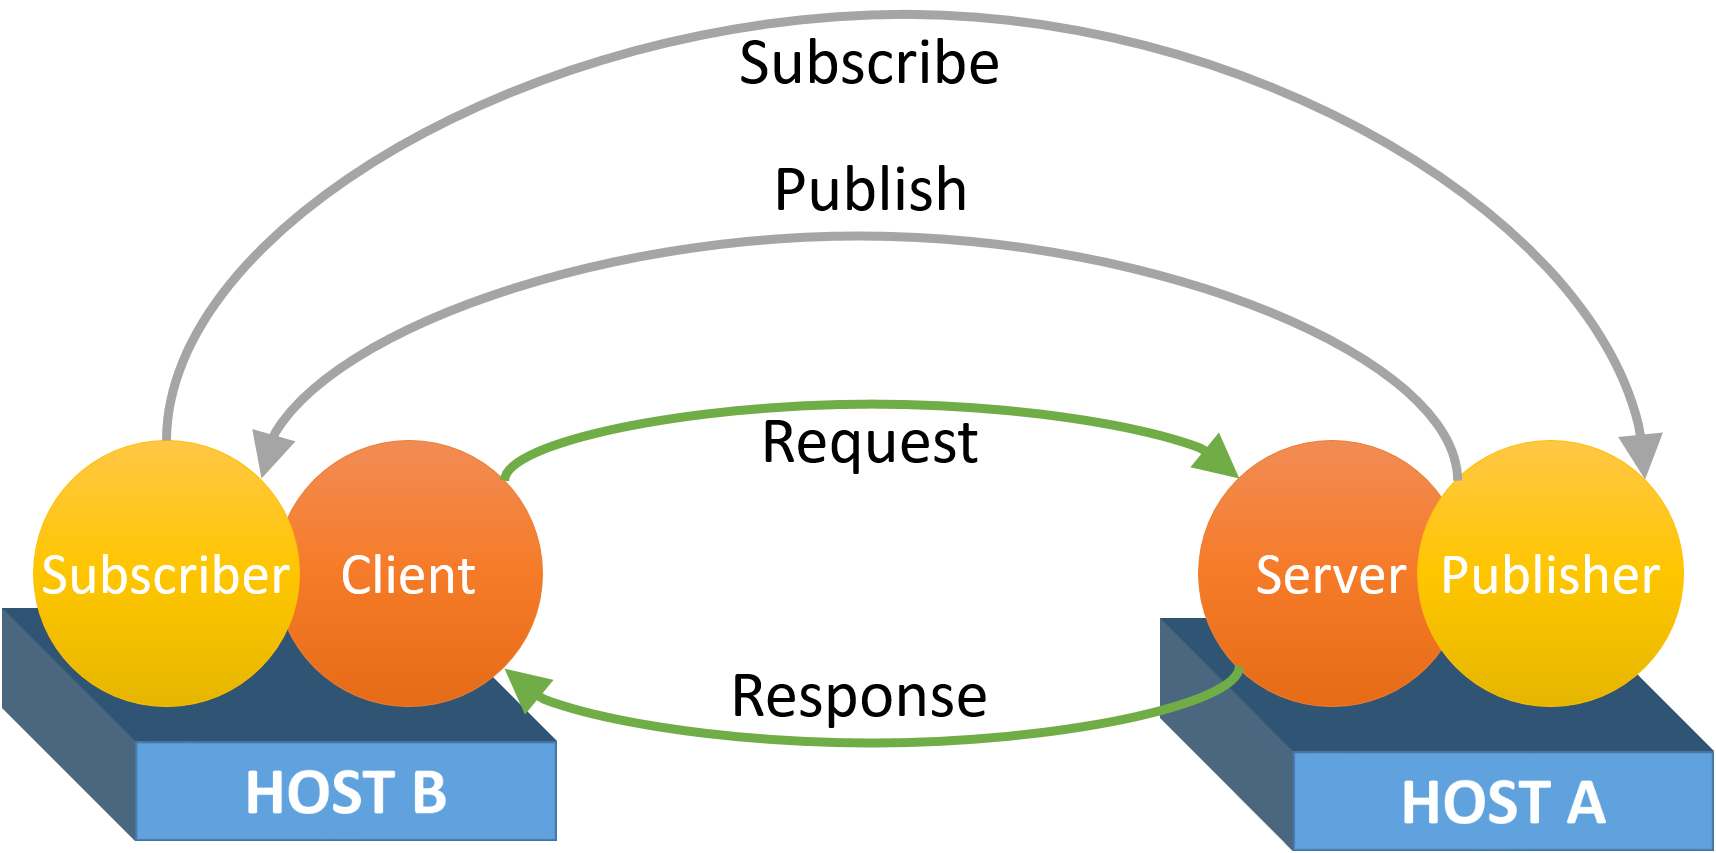
\includegraphics[width=.6\textwidth]{Paradigm}
\centering
\end{figure}

\end{frame}

% INTEGRATION TESTING
\section{Integration Testing}

\subsection{Overall View on Integration Components}

% Define block styles
\tikzstyle{block} = [rectangle, draw, fill=gray!20,
    text width=6em, text centered, rounded corners, minimum height=4em]
    
\tikzstyle{hiddenblock} = [rectangle, draw, fill=gray!5, text = gray!50, draw=gray!50,
    text width=6em, text centered, rounded corners, minimum height=4em]

\tikzstyle{driverblock} = [rectangle, draw, fill=red!20, 
    text width=6em, text centered, rounded corners, minimum height=4em]

\tikzstyle{testedblock} = [rectangle, draw, fill=green!20, 
    text width=6em, text centered, rounded corners, minimum height=4em]
    
\tikzstyle{stubblock} = [rectangle, draw, fill=blue!20, 
    text width=6em, text centered, rounded corners, minimum height=4em]

\tikzstyle{line} = [draw, -latex']
\tikzstyle{hiddenline} = [draw=gray!50, text=gray!50, -latex']
\tikzstyle{testedline} = [draw=green, -latex', line width = 0.35mm]

\begin{frame}{\currentname}

\begin{columns}[c]
  \begin{column}{.5\textwidth}
    \vbox to .8\textheight{
        
        \vfill
        
        \textbf{Strategy:} \newline
        Bottom Up approach but... not pure!

        \vfill
    
        Test the integration starting from the application logic and finishing with the graphical user interface

        \vfill

         Not always possible due to the presence of complex interconnections
         
         \vfill
         
         Some stubs are needed
         
         \vfill
         
        }

  \end{column}
  \begin{column}{.5\textwidth}
    \begin{figure}[H]
    \begin{tikzpicture}[node distance = 2cm, auto, scale=0.5, transform shape]
        % Place nodes
        \node [block] (db) {Database};
        \node [block, right of=db, above of=db] (account) {Account Manager};
        \node [block, right of=db, below of=db, fill=yellow!20] (application) {Application};
        \node [block, right of=db, node distance = 5cm] (appgui) {Mobile Application};
        \node [block, right of=appgui, text width=8em, node distance = 3.5cm] (webgui) {Web Application};
        % Draw edges
        \path [line] (db) -- node {IT7} (account);
        \path [line] (db) -- node {IT8} (application);
        \path [line] (account) -- node {IT9} (application);
        \path [line] (application) -- node {IT11} (appgui);
        \path [line] (application) -| node [near start] {IT11}  (webgui);
        \path [line] (account) -| node [near start] {IT10} (webgui);
        \path [line] (account) -- node {IT10} (appgui);
    \end{tikzpicture}
    \end{figure}
    \begin{figure}[H]
    \begin{tikzpicture}[node distance = 2.3cm, auto, scale=0.5, transform shape]
        \draw [color=gray,thick, rounded corners, fill=yellow!20](-1.7,-3.5) rectangle (7.7,3.5);
        \node at (-1.5,3.7) [above=0mm, right=0mm] {\textsc{Application}};
        % Place nodes
        \node [block] (position) {Position Manager};
        \node [block, right of=position, node distance = 6cm] (notification) {Notification Manager};
        \node [block, below of=position] (queue) {Queue Manager};
        \node [block, below of=notification] (call) {Call Manager};
        \node [block, above of=notification] (reservation) {Reservation Manager};
        % Draw edges
        \path [line] (notification) -- node {IT6} (call);
        \path [line] (position) -- node {IT1} (queue);
        \path [line] (position) -- node {IT15} (call);
        \path [line] (queue) -- node {IT4} (call);
        \path [line] (notification) -- node {IT3} (reservation);
        \path [line] (position) -- node {IT2} (reservation);
    \end{tikzpicture}
    \end{figure}
  \end{column}
\end{columns}

\end{frame}

\subsection{Integration Steps}

\begin{frame}{\currentname}
	
\framesubtitle{Application}
	
\begin{figure}[H]
	\begin{tikzpicture}[node distance = 3cm, auto, scale=0.8, transform shape]
	\draw [color=gray,thick, rounded corners, fill=yellow!20](-1.5,-4) rectangle (13.5,4);
	\node at (-1.5,4.3) [above=0mm, right=0mm] {\textsc{Application}};
	% Place nodes
	\node [hiddenblock] (position) {Position Manager};
	\node [hiddenblock, right of=position, node distance = 6cm] (notification) {Notification Manager};
	\node [hiddenblock, below of=notification, left of=notification] (queue) {Queue Manager};
	\node [hiddenblock, right of=queue, node distance = 9cm] (call) {Call Manager};
	\node [hiddenblock, above of=notification, right of=notification] (reservation) {Reservation Manager};
	% Draw edges
	\path [hiddenline] (notification) -- node {IT6} (call);
	\path [hiddenline] (position) -- node {IT1} (queue);
	\path [hiddenline] (position) -- node {IT15} (call);
	\path [hiddenline] (queue) -- node {IT4} (call);
	\path [hiddenline] (notification) -- node {IT3} (reservation);
	\path [hiddenline] (position) -- node {IT2} (reservation);
	\end{tikzpicture}
\end{figure}

\end{frame}

\begin{frame}{\currentname{} - IT1}
\framesubtitle{Application: Integration between Position Manager and Queue Manager}
\begin{figure}[H]
\begin{tikzpicture}[node distance = 3cm, auto, scale=0.8, transform shape]
    \draw [color=gray,thick, rounded corners, fill=yellow!20](-1.5,-4) rectangle (13.5,4);
    \node at (-1.5,4.3) [above=0mm, right=0mm] {\textsc{Application}};
    % Place nodes
    \node [block] (position) {Position Manager};
    \node [hiddenblock, right of=position, node distance = 6cm] (notification) {Notification Manager};
    \node [block, below of=notification, left of=notification] (queue) {Queue Manager};
    \node [hiddenblock, right of=queue, node distance = 9cm] (call) {Call Manager};
    \node [hiddenblock, above of=notification, right of=notification] (reservation) {Reservation Manager};
    % Draw edges
    \path [hiddenline] (notification) -- node {IT6} (call);
    \path [line] (position) -- node {IT1} (queue);
    \path [hiddenline] (position) -- node {IT15} (call);
    \path [hiddenline] (queue) -- node {IT4} (call);
    \path [hiddenline] (notification) -- node {IT3} (reservation);
    \path [hiddenline] (position) -- node {IT2} (reservation);

	%Additions
	\onslide<2->{
	    \node [driverblock, below of=position] (driver) {Driver};
	    \path [line] (queue) -- (driver);
	}
\end{tikzpicture}
\end{figure}
\end{frame}

\begin{frame}{\currentname{} - IT2}
	\framesubtitle{Application: Integration between Position Manager and Reservation Manager}
	\begin{figure}[H]
		\begin{tikzpicture}[node distance = 3cm, auto, scale=0.8, transform shape]
		\draw [color=gray,thick, rounded corners, fill=yellow!20](-1.5,-4) rectangle (13.5,4);
		\node at (-1.5,4.3) [above=0mm, right=0mm] {\textsc{Application}};
		% Place nodes
		\node [block] (position) {Position Manager};
		\node [hiddenblock, right of=position, node distance = 6cm] (notification) {Notification Manager};
		\node [hiddenblock, below of=notification, left of=notification] (queue) {Queue Manager};
		\node [hiddenblock, right of=queue, node distance = 9cm] (call) {Call Manager};
		\node [block, above of=notification, right of=notification] (reservation) {Reservation Manager};

		% Draw edges
		\path [hiddenline] (notification) -- node {IT6} (call);
		\path [testedline] (position) -- node {IT1} (queue);
		\path [hiddenline] (position) -- node {IT15} (call);
		\path [hiddenline] (queue) -- node {IT4} (call);
		\path [hiddenline] (notification) -- node {IT3} (reservation);
		\path [line] (position) -- node {IT2} (reservation);
		
		% Additions
		\onslide<2->{
			\node [stubblock, below of=reservation] (stub) {Stub for Notification Manager};
			\path [line] (stub) -- (reservation);
		}
		\onslide<3->{
			\node [driverblock, right of=reservation] (driver) {Driver};
			\path [line] (reservation) -- (driver);
		}
		\end{tikzpicture}
	\end{figure}
\end{frame}

\begin{frame}{\currentname{} - IT3}
	\framesubtitle{Application: Integration between Notification Manager and Reservation Manager}
	\begin{figure}[H]
		\begin{tikzpicture}[node distance = 3cm, auto, scale=0.8, transform shape]
		\draw [color=gray,thick, rounded corners, fill=yellow!20](-1.5,-4) rectangle (13.5,4);
		\node at (-1.5,4.3) [above=0mm, right=0mm] {\textsc{Application}};
		% Place nodes
		\node [testedblock] (position) {Position Manager};
		\node [block, right of=position, node distance = 6cm] (notification) {Notification Manager};
		\node [hiddenblock, below of=notification, left of=notification] (queue) {Queue Manager};
		\node [hiddenblock, right of=queue, node distance = 9cm] (call) {Call Manager};
		\node [block, above of=notification, right of=notification] (reservation) {Reservation Manager};
		
		% Draw edges
		\path [hiddenline] (notification) -- node {IT6} (call);
		\path [testedline] (position) -- node {IT1} (queue);
		\path [hiddenline] (position) -- node {IT15} (call);
		\path [hiddenline] (queue) -- node {IT4} (call);
		\path [line] (notification) -- node {IT3} (reservation);
		\path [testedline] (position) -- node {IT2} (reservation);
		
		% Additions
		\onslide<2->{
			\node [driverblock, right of=reservation] (driver) {Driver};
			\path [line] (reservation) -- (driver);
		}
		\end{tikzpicture}
	\end{figure}
\end{frame}

\begin{frame}{\currentname{} - IT4}
	\framesubtitle{Application: Integration between Queue Manager and Call Manager}
	\begin{figure}[H]
		\begin{tikzpicture}[node distance = 3cm, auto, scale=0.8, transform shape]
		\draw [color=gray,thick, rounded corners, fill=yellow!20](-1.5,-4) rectangle (13.5,4);
		\node at (-1.5,4.3) [above=0mm, right=0mm] {\textsc{Application}};
		% Place nodes
		\node [testedblock] (position) {Position Manager};
		\node [hiddenblock, right of=position, node distance = 6cm] (notification) {Notification Manager};
		\node [block, below of=notification, left of=notification] (queue) {Queue Manager};
		\node [block, right of=queue, node distance = 9cm] (call) {Call Manager};
		\node [hiddenblock, above of=notification] (reservation) {Reservation Manager};
		
		% Draw edges
		\path [hiddenline] (notification) -- node {IT6} (call);
		\path [testedline] (position) -- node {IT1} (queue);
		\path [hiddenline] (position) -- node {IT15} (call);
		\path [line] (queue) -- node {IT4} (call);
		\path [testedline] (notification) -- node {IT3} (reservation);
		\path [testedline] (position) -- node {IT2} (reservation);
		
		% Additions
		\onslide<2->{
			\node [stubblock, right of=reservation] (stub) {Stub for Notification Manager};
			\path [line] (stub) -- (call);
		}
		\onslide<3->{
			\node [stubblock, right of=notification] (stub1) {Stub for Position Manager};
			\path [line] (stub1) -- (call);
		}
		\onslide<4->{
			\node [driverblock, above of=call] (driver) {Driver};
			\path [line] (call) -- (driver);
		}
		\end{tikzpicture}
	\end{figure}
\end{frame}

\begin{frame}{\currentname{} - IT5}
	\framesubtitle{Application: Integration between Position Manager and Call Manager}
	\begin{figure}[H]
		\begin{tikzpicture}[node distance = 3cm, auto, scale=0.8, transform shape]
		\draw [color=gray,thick, rounded corners, fill=yellow!20](-1.5,-4) rectangle (13.5,4);
		\node at (-1.5,4.3) [above=0mm, right=0mm] {\textsc{Application}};
		% Place nodes
		\node [block] (position) {Position Manager};
		\node [hiddenblock, right of=position, node distance = 6cm] (notification) {Notification Manager};
		\node [testedblock, below of=notification, left of=notification] (queue) {Queue Manager};
		\node [block, right of=queue, node distance = 9cm] (call) {Call Manager};
		\node [hiddenblock, above of=notification, right of=notification] (reservation) {Reservation Manager};
		
		% Draw edges
		\path [hiddenline] (notification) -- node {IT6} (call);
		\path [testedline] (position) -- node {IT1} (queue);
		\path [line] (position) -- node {IT15} (call);
		\path [testedline] (queue) -- node {IT4} (call);
		\path [testedline] (notification) -- node {IT3} (reservation);
		\path [testedline] (position) -- node {IT2} (reservation);
		
		% Additions
		\onslide<2->{
			\node [stubblock, below of=reservation] (stub) {Stub for Notification Manager};
			\path [line] (stub) -- (call);
		}
		\onslide<3->{
			\node [driverblock, right of=stub] (driver) {Driver};
			\path [line] (call) -- (driver);
		}
		\end{tikzpicture}
	\end{figure}
\end{frame}

\begin{frame}{\currentname{} - IT6}
	\framesubtitle{Application: Integration between Notification Manager and Call Manager}
	\begin{figure}[H]
		\begin{tikzpicture}[node distance = 3cm, auto, scale=0.8, transform shape]
		\draw [color=gray,thick, rounded corners, fill=yellow!20](-1.5,-4) rectangle (13.5,4);
		\node at (-1.5,4.3) [above=0mm, right=0mm] {\textsc{Application}};
		% Place nodes
		\node [testedblock] (position) {Position Manager};
		\node [block, right of=position, node distance = 6cm] (notification) {Notification Manager};
		\node [testedblock, below of=notification, left of=notification] (queue) {Queue Manager};
		\node [block, right of=queue, node distance = 9cm] (call) {Call Manager};
		\node [hiddenblock, above of=notification, right of=notification] (reservation) {Reservation Manager};
		
		% Draw edges
		\path [line] (notification) -- node {IT6} (call);
		\path [testedline] (position) -- node {IT1} (queue);
		\path [testedline] (position) -- node {IT15} (call);
		\path [testedline] (queue) -- node {IT4} (call);
		\path [testedline] (notification) -- node {IT3} (reservation);
		\path [testedline] (position) -- node {IT2} (reservation);
		
		% Additions
		\onslide<2->{
			\node [driverblock, right of=stub] (driver) {Driver};
			\path [line] (call) -- (driver);
		}
		\end{tikzpicture}
	\end{figure}
\end{frame}

\begin{frame}{\currentname{}}
	\framesubtitle{Application Tested!}
	\begin{figure}[H]
		\begin{tikzpicture}[node distance = 3cm, auto, scale=0.8, transform shape]
		\draw [color=gray,thick, rounded corners, fill=yellow!20](-1.5,-4) rectangle (13.5,4);
		\node at (-1.5,4.3) [above=0mm, right=0mm] {\textsc{Application}};
		% Place nodes
		\node [testedblock] (position) {Position Manager};
		\node [testedblock, right of=position, node distance = 6cm] (notification) {Notification Manager};
		\node [testedblock, below of=notification, left of=notification] (queue) {Queue Manager};
		\node [testedblock, right of=queue, node distance = 9cm] (call) {Call Manager};
		\node [testedblock, above of=notification, right of=notification] (reservation) {Reservation Manager};
		
		% Draw edges
		\path [testedline] (notification) -- node {IT6} (call);
		\path [testedline] (position) -- node {IT1} (queue);
		\path [testedline] (position) -- node {IT15} (call);
		\path [testedline] (queue) -- node {IT4} (call);
		\path [testedline] (notification) -- node {IT3} (reservation);
		\path [testedline] (position) -- node {IT2} (reservation);
		
		\end{tikzpicture}
	\end{figure}
\end{frame}

\begin{frame}{\currentname}
	\framesubtitle{Global}
	\begin{figure}[H]
	\begin{tikzpicture}[node distance = 2.5cm, auto]
	% Place nodes
	\node [hiddenblock] (db) {Database};
	\node [hiddenblock, right of=db, above of=db] (account) {Account Manager};
	\node [hiddenblock, right of=db, below of=db, fill=yellow!20] (application) {Application};
	\node [hiddenblock, right of=application, above of=application] (appgui) {Mobile Application};
	\node [hiddenblock, right of=appgui, text width=8em, node distance = 3.5cm] (webgui) {Web Application};
	% Draw edges
	\path [hiddenline] (db) -- node {IT7} (account);
	\path [hiddenline] (db) -- node {IT8} (application);
	\path [hiddenline] (account) -- node {IT9} (application);
	\path [hiddenline] (application) -- node {IT11} (appgui);
	\path [hiddenline] (application) -| node [near start] {IT11}  (webgui);
	\path [hiddenline] (account) -| node [near start] {IT10} (webgui);
	\path [hiddenline] (account) -- node {IT10} (appgui);
	\end{tikzpicture}
\end{figure}
\end{frame}

\begin{frame}{\currentname{} - IT7}
	\framesubtitle{Global: Integration between Database and Account Manager}
	\begin{figure}[H]
		\begin{tikzpicture}[node distance = 2.5cm, auto]
		% Place nodes
		\node [block] (db) {Database};
		\node [block, right of=db, above of=db] (account) {Account Manager};
		\node [hiddenblock, right of=db, below of=db, fill=yellow!20] (application) {Application};
		\node [hiddenblock, right of=application, above of=application] (appgui) {Mobile Application};
		\node [hiddenblock, right of=appgui, text width=8em, node distance = 3.5cm] (webgui) {Web Application};
		% Draw edges
		\path [line] (db) -- node {IT7} (account);
		\path [hiddenline] (db) -- node {IT8} (application);
		\path [hiddenline] (account) -- node {IT9} (application);
		\path [hiddenline] (application) -- node {IT11} (appgui);
		\path [hiddenline] (application) -- node [near start] {IT11}  (webgui);
		\path [hiddenline] (account) -- node [near start] {IT10} (webgui);
		\path [hiddenline] (account) -- node {IT10} (appgui);
		
		% Additions
		\onslide<2->{
			\node [driverblock, above of=webgui] (driver) {Driver};
			\path [line] (account) -- (driver);
		}
		\end{tikzpicture}
	\end{figure}
\end{frame}

\begin{frame}{\currentname{} - IT8}
	\framesubtitle{Global: Integration between Database and Application}
	\begin{figure}[H]
		\begin{tikzpicture}[node distance = 2.5cm, auto]
		% Place nodes
		\node [block] (db) {Database};
		\node [hiddenblock, right of=db, above of=db] (account) {Account Manager};
		\node [block, right of=db, below of=db, fill=yellow!20] (application) {Application};
		\node [hiddenblock, right of=application, above of=application] (appgui) {Mobile Application};
		\node [hiddenblock, right of=appgui, text width=8em, node distance = 3.5cm] (webgui) {Web Application};
		% Draw edges
		\path [testedline] (db) -- node {IT7} (account);
		\path [line] (db) -- node {IT8} (application);
		\path [hiddenline] (account) -- node {IT9} (application);
		\path [hiddenline] (application) -- node {IT11} (appgui);
		\path [hiddenline] (application) -- node [near start] {IT11}  (webgui);
		\path [hiddenline] (account) -- node [near start] {IT10} (webgui);
		\path [hiddenline] (account) -- node {IT10} (appgui);
		
		% Additions
		\onslide<2->{
				\node [stubblock, left of=application] (stub) {Stub for Account Manager};
				\path [line] (stub) -- (application);
			}
		\onslide<3->{
			\node [driverblock, below of=webgui] (driver) {Driver};
			\path [line] (application) -- (driver);
		}
		\end{tikzpicture}
	\end{figure}
\end{frame}

\begin{frame}{\currentname{} - IT9}
	\framesubtitle{Global: Integration between Account Manager and Application}
	\begin{figure}[H]
		\begin{tikzpicture}[node distance = 2.5cm, auto]
		% Place nodes
		\node [testedblock] (db) {Database};
		\node [block, right of=db, above of=db] (account) {Account Manager};
		\node [block, right of=db, below of=db, fill=yellow!20] (application) {Application};
		\node [hiddenblock, right of=application, above of=application] (appgui) {Mobile Application};
		\node [hiddenblock, right of=appgui, text width=8em, node distance = 3.5cm] (webgui) {Web Application};
		% Draw edges
		\path [testedline] (db) -- node {IT7} (account);
		\path [testedline] (db) -- node {IT8} (application);
		\path [line] (account) -- node {IT9} (application);
		\path [hiddenline] (application) -- node {IT11} (appgui);
		\path [hiddenline] (application) -- node [near start] {IT11}  (webgui);
		\path [hiddenline] (account) -- node [near start] {IT10} (webgui);
		\path [hiddenline] (account) -- node {IT10} (appgui);
		
		% Additions
		\onslide<2->{
			\node [driverblock, below of=webgui] (driver) {Driver};
			\path [line] (application) -- (driver);
		}
		\end{tikzpicture}
	\end{figure}
\end{frame}

\begin{frame}{\currentname{} - IT10}
	\framesubtitle{Global: Integration between Account Manager and User Interface}
	\begin{figure}[H]
		\begin{tikzpicture}[node distance = 2.5cm, auto]
		% Place nodes
		\node [testedblock] (db) {Database};
		\node [block, right of=db, above of=db] (account) {Account Manager};
		\node [hiddenblock, right of=db, below of=db, fill=yellow!20] (application) {Application};
		\node [block, right of=application, above of=application] (appgui) {Mobile Application};
		\node [block, right of=appgui, text width=8em, node distance = 3.5cm] (webgui) {Web Application};
		% Draw edges
		\path [testedline] (db) -- node {IT7} (account);
		\path [testedline] (db) -- node {IT8} (application);
		\path [testedline] (account) -- node {IT9} (application);
		\path [hiddenline] (application) -- node {IT11} (appgui);
		\path [hiddenline] (application) -- node [near start] {IT11}  (webgui);
		\path [line] (account) -- node [near start] {IT10} (webgui);
		\path [line] (account) -- node {IT10} (appgui);
		
		% Additions
		\onslide<2->{
			\node [stubblock, above of=webgui] (stub) {Stub for Application};
			\path [line] (stub) -- (appgui);
			\path [line] (stub) -- (webgui);
		}
		\onslide<3->{
			\node [driverblock, below of=webgui] (driver) {Driver (human user)};
			\path [line] (appgui) -- (driver);
			\path [line] (webgui) -- (driver);
		}
		\end{tikzpicture}
	\end{figure}
\end{frame}

\begin{frame}{\currentname{} - IT11}
	\framesubtitle{Global: Integration between Application and User Interface}
	\begin{figure}[H]
		\begin{tikzpicture}[node distance = 2.5cm, auto]
		% Place nodes
		\node [testedblock] (db) {Database};
		\node [testedblock, right of=db, above of=db] (account) {Account Manager};
		\node [block, right of=db, below of=db, fill=yellow!20] (application) {Application};
		\node [block, right of=application, above of=application] (appgui) {Mobile Application};
		\node [block, right of=appgui, text width=8em, node distance = 3.5cm] (webgui) {Web Application};
		% Draw edges
		\path [testedline] (db) -- node {IT7} (account);
		\path [testedline] (db) -- node {IT8} (application);
		\path [testedline] (account) -- node {IT9} (application);
		\path [line] (application) -- node {IT11} (appgui);
		\path [line] (application) -- node [near start] {IT11}  (webgui);
		\path [testedline] (account) -- node [near start] {IT10} (webgui);
		\path [testedline] (account) -- node {IT10} (appgui);
		
		% Additions
		\onslide<2->{
			\node [driverblock, below of=webgui] (driver) {Driver (human user)};
			\path [line] (appgui) -- (driver);
			\path [line] (webgui) -- (driver);
		}
		\end{tikzpicture}
	\end{figure}
\end{frame}

\begin{frame}{\currentname{}}
	\framesubtitle{Whole System Tested!}
	\begin{figure}[H]
		\begin{tikzpicture}[node distance = 2.5cm, auto]
		% Place nodes
		\node [testedblock] (db) {Database};
		\node [testedblock, right of=db, above of=db] (account) {Account Manager};
		\node [testedblock, right of=db, below of=db] (application) {Application};
		\node [testedblock, right of=application, above of=application] (appgui) {Mobile Application};
		\node [testedblock, right of=appgui, text width=8em, node distance = 3.5cm] (webgui) {Web Application};
		% Draw edges
		\path [testedline] (db) -- node {IT7} (account);
		\path [testedline] (db) -- node {IT8} (application);
		\path [testedline] (account) -- node {IT9} (application);
		\path [testedline] (application) -- node {IT11} (appgui);
		\path [testedline] (application) -| node [near start] {IT11}  (webgui);
		\path [testedline] (account) -| node [near start] {IT10} (webgui);
		\path [testedline] (account) -- node {IT10} (appgui);
		\end{tikzpicture}
	\end{figure}
\end{frame}

% PROJECT PLANNING
\section{Project Planning}
\subsection{Function Points}

\begin{frame}{\currentname}

\begin{figure}[H]
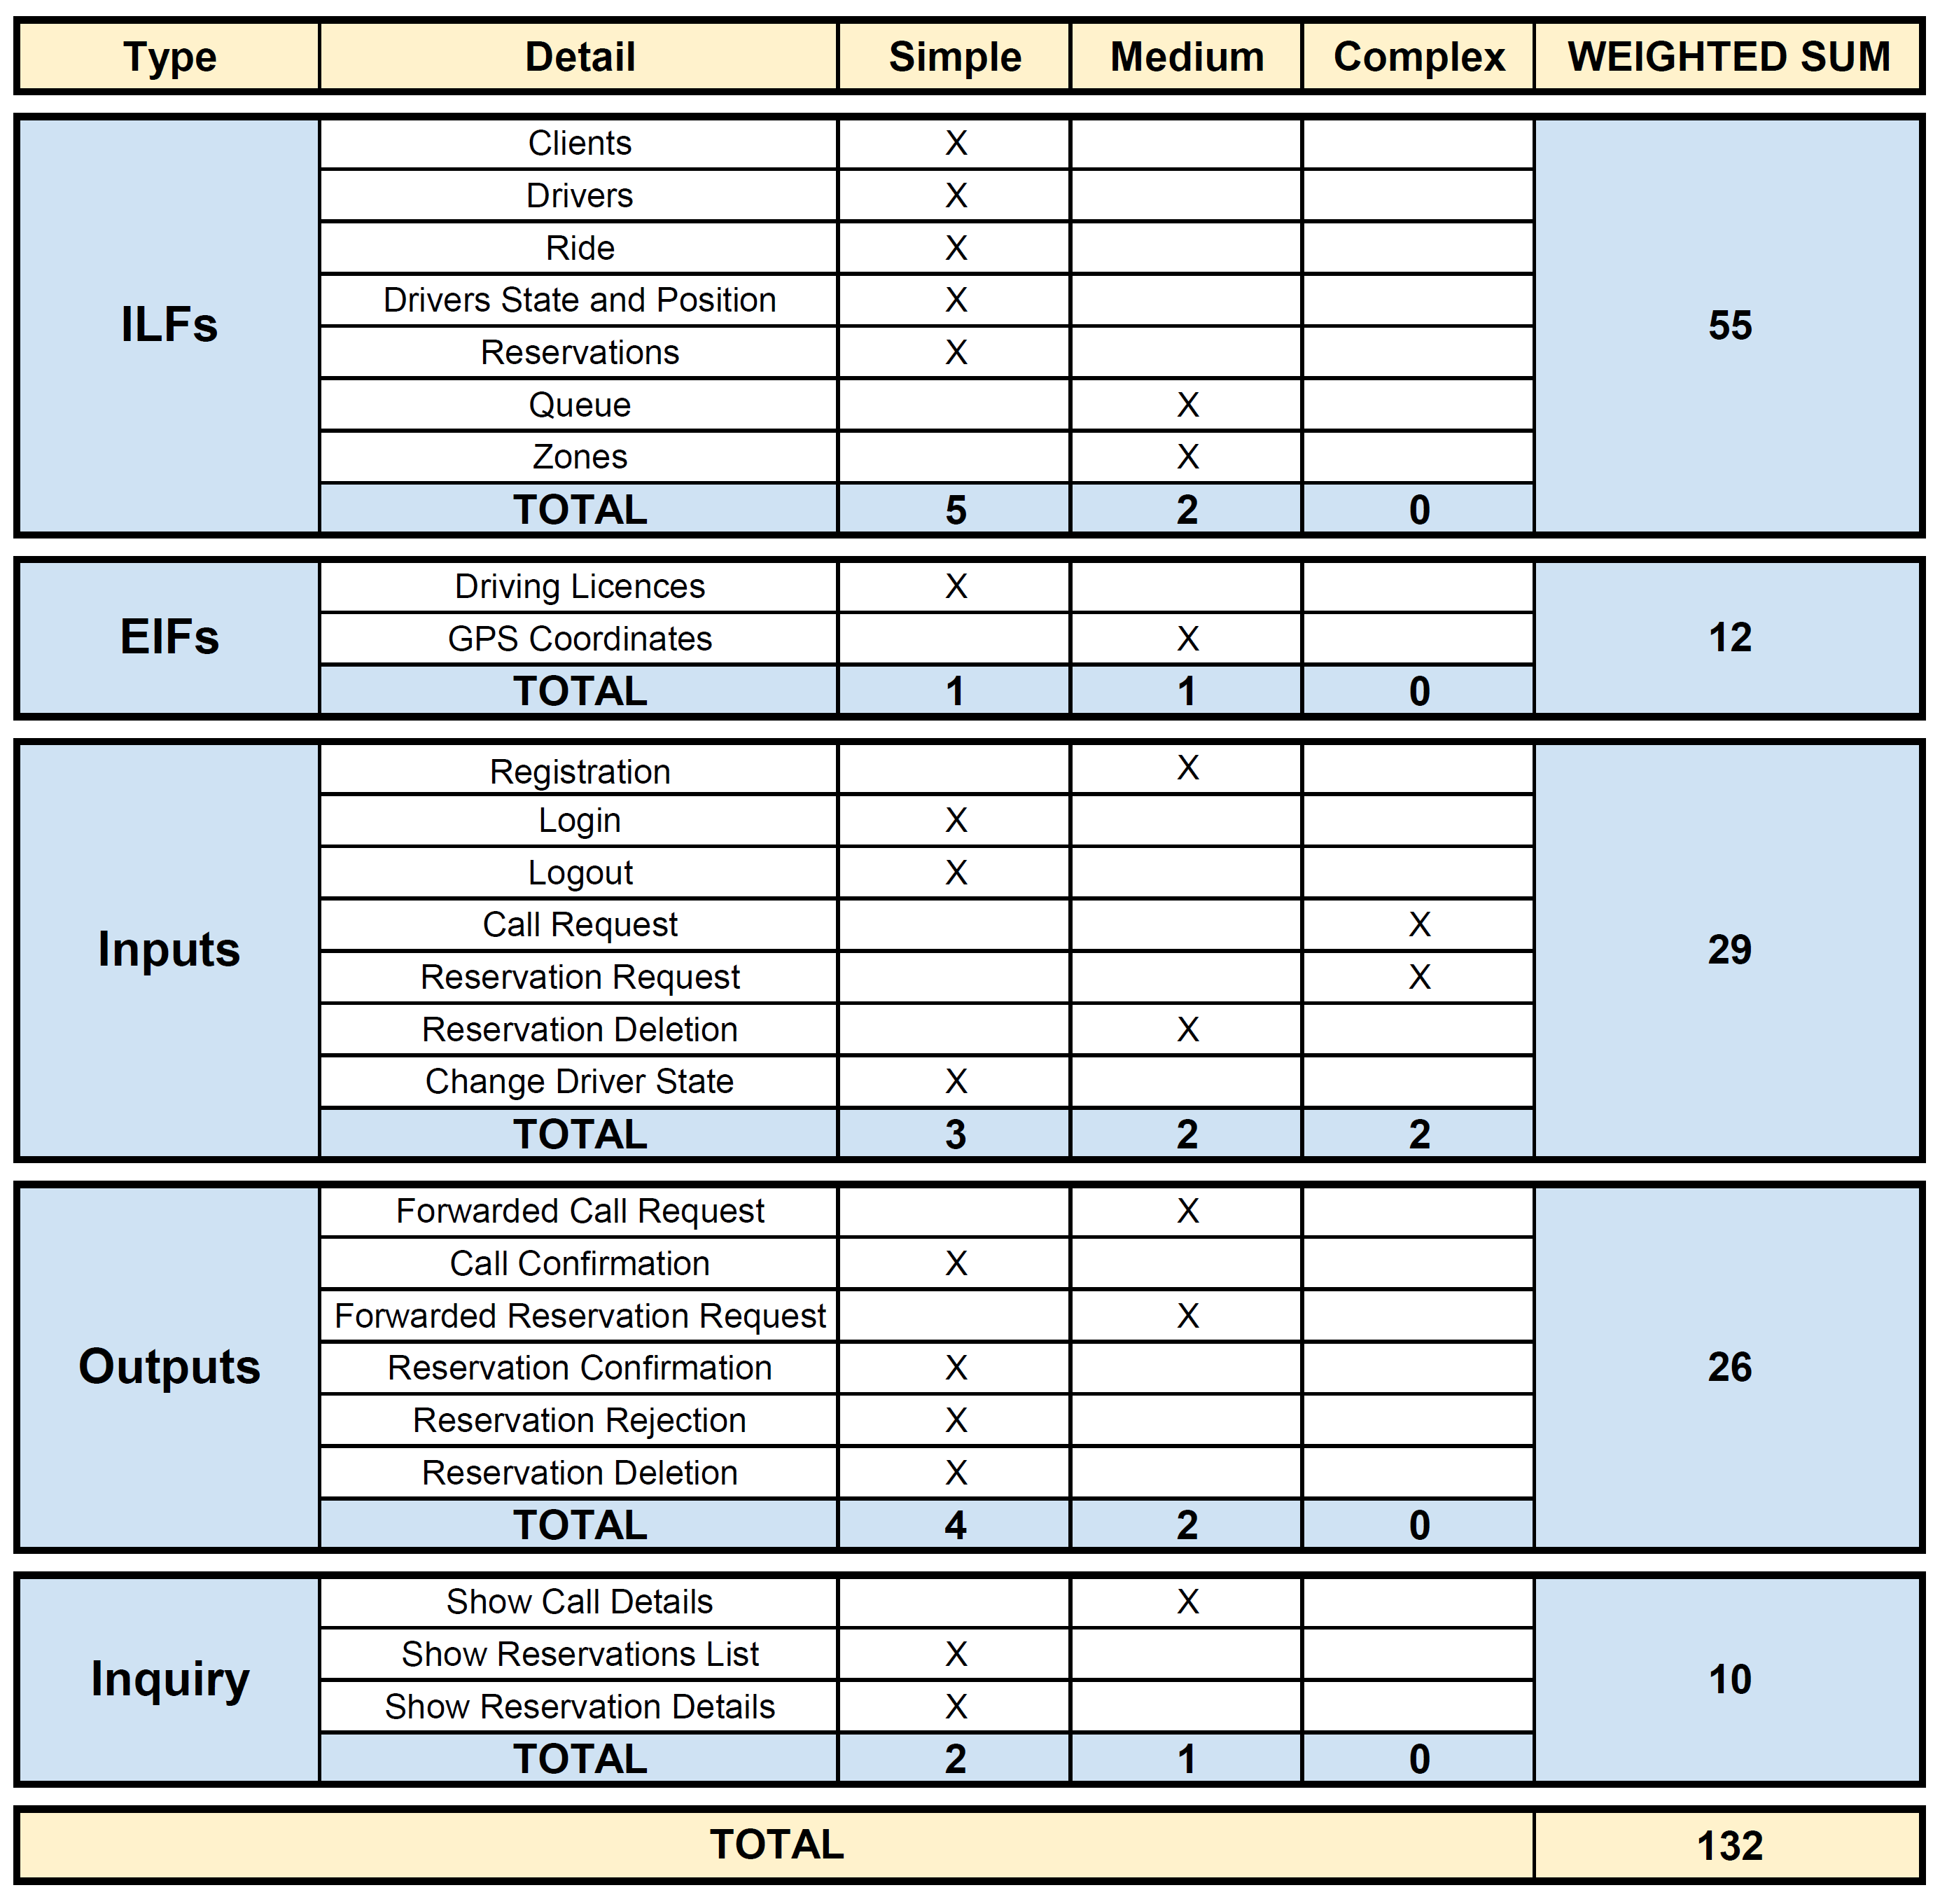
\includegraphics[height=.8\textheight]{FunctionPoints}
\centering
\end{figure}

\end{frame}

\subsection{COCOMO}

\begin{frame}{\currentname}

\begin{figure}[H]
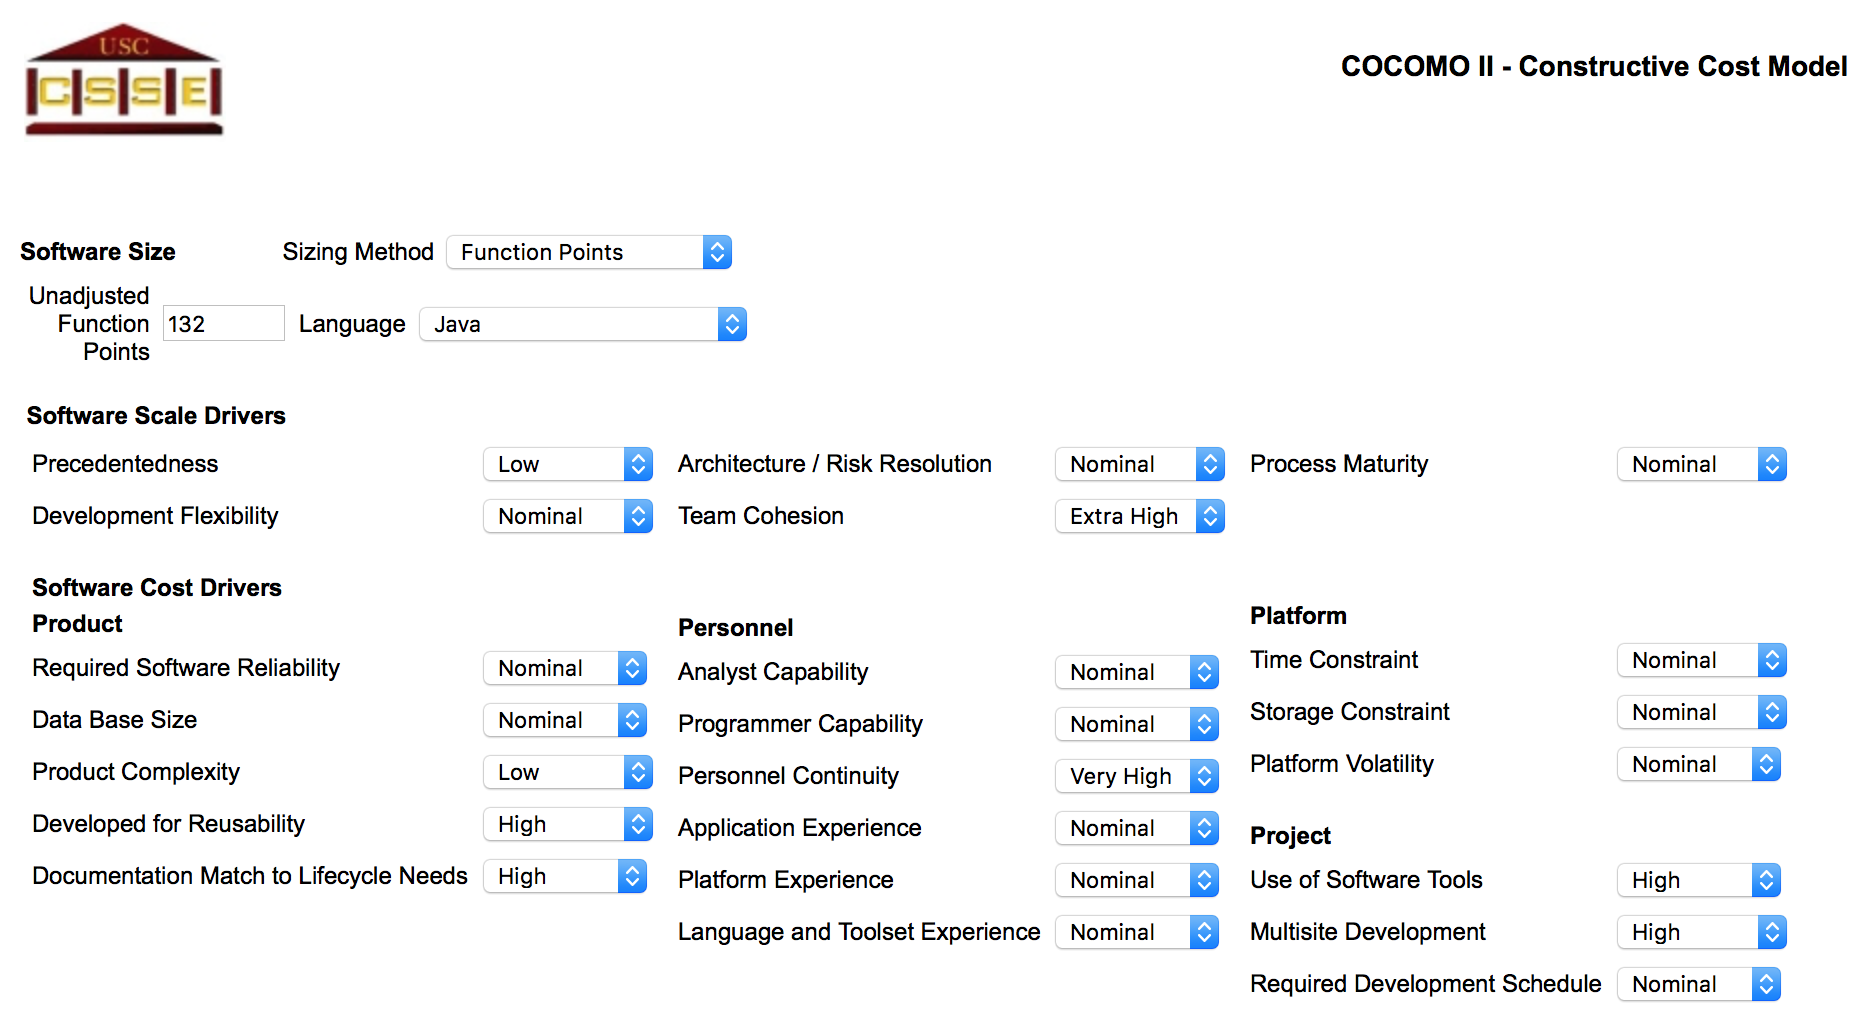
\includegraphics[height=.6\textheight]{COCOMO-Settings}
\centering
\end{figure}

\end{frame}
\begin{frame}{\currentname}

\begin{figure}[H]
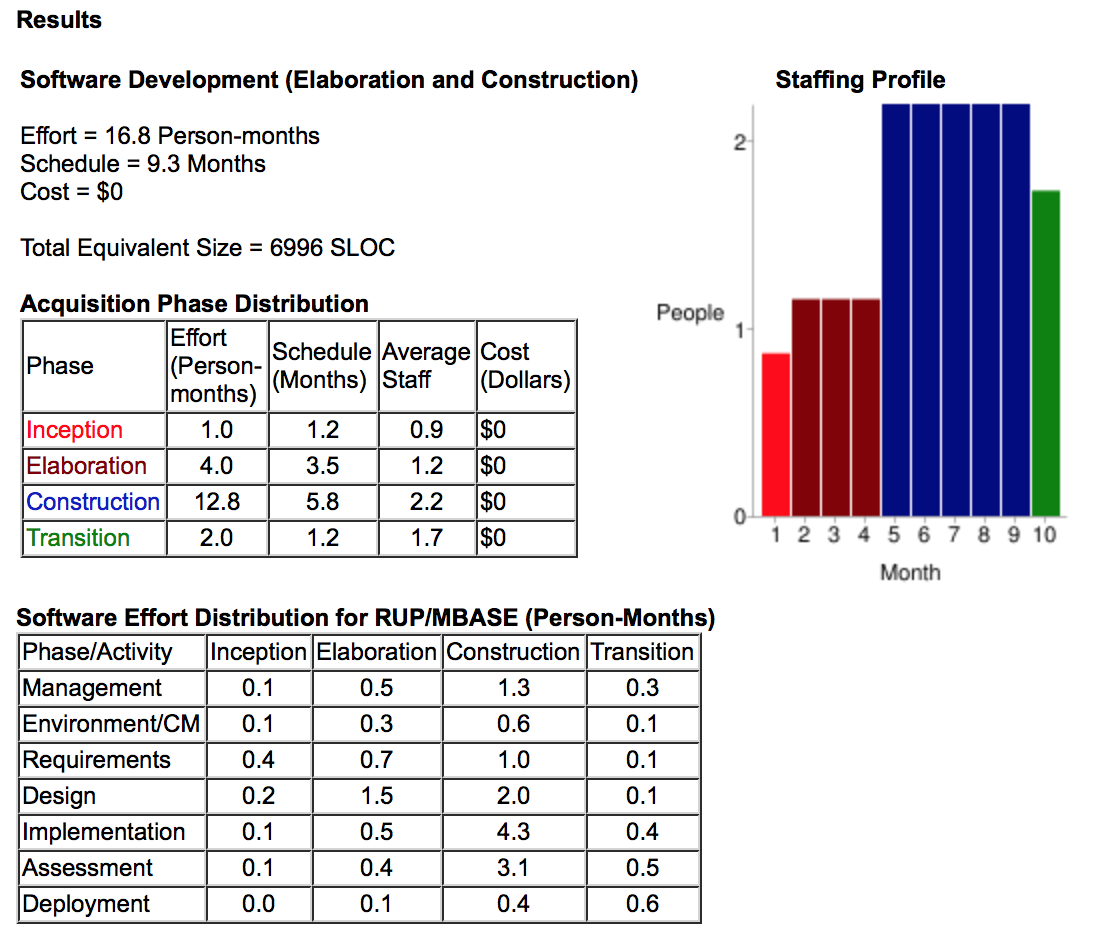
\includegraphics[height=.8\textheight]{COCOMO-Results}
\centering
\end{figure}

\end{frame}

\subsection{Gantt Chart}
\begin{frame}{\currentname{}}
\begin{columns}[c]
  \begin{column}{.5\textwidth}
	    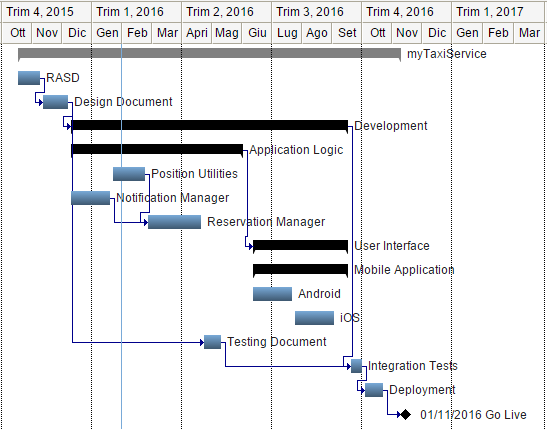
\includegraphics[width=\textwidth]{GANTT_CHART_JACOPO}
		\centering
		\newline
		Jacopo's tasks
  \end{column}
  \begin{column}{.5\textwidth}
    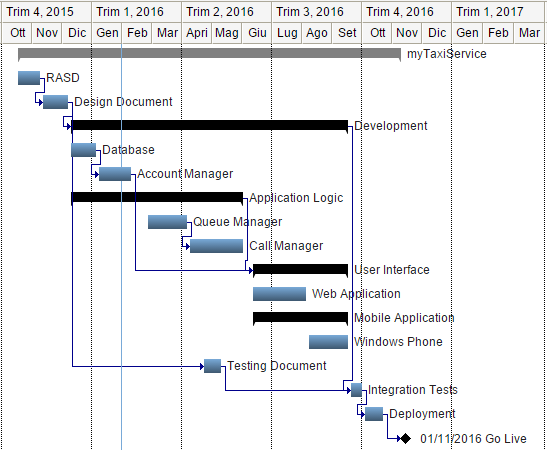
\includegraphics[width=\textwidth]{GANTT_CHART_LUCA}
		\centering
		\newline
		Luca's tasks
  \end{column}
\end{columns}
\end{frame}

% END

\begin{frame}{Questions?}
\begin{figure}[H]

\includegraphics[height=.6\textheight]{questions}
\centering
\end{figure}
\end{frame}

\end{document}